\documentclass{acm_proc_article-sp}

\usepackage{cite}
\usepackage{graphicx}
%\usepackage[cmex10]{amsmath}
%\usepackage{amssymb}
%\usepackage{array}
\usepackage{url}
\usepackage{listings}

\lstdefinestyle{FortranLike}{float,frame=lines,language=Fortran,commentstyle=\ttfamily,basicstyle=\ttfamily}
\lstdefinestyle{CLike}{float,frame=lines,language=C,commentstyle=\ttfamily,basicstyle=\ttfamily}
\lstdefinestyle{NoFloatCLike}{frame=lines,language=C,commentstyle=\ttfamily,basicstyle=\ttfamily}

\begin{document}

\title{Locally-Oriented Programming: A stunningly simple programming model for GPU programming in Fortran and C++}

\numberofauthors{4}

\author{
% 1st. author
\alignauthor
Craig E Rasmussen\\
       \affaddr{Los Alamos National Laboratory}\\
%       \affaddr{CCS-7, MS B287}\\
       \affaddr{Los Alamos, NM 87545}\\
       \email{crasmussen@lanl.gov}
% 2nd. author
\alignauthor
Matthew J. Sottile\\
       \affaddr{Galois, Inc.}\\
%       \affaddr{421 SW 6th Ave. Suite 300}\\
       \affaddr{Portland, OR 97204}\\
       \email{mjsottile@computer.org}
% 3rd. author
\alignauthor
Dan Nagle\\
       \email{dannagle@verizon.net}
% 4th. author
\alignauthor
Daniel Quinlan\\
       \affaddr{Lawrence Livermore National Laboratory}\\
       \email{dquinlan@llnl.gov}
}

\maketitle

\begin{abstract}
Emerging GPU architectures for high performance computing are well suited to a
data-parallel programming model.  However, programming for these architectures
currently requires learning a new language, e.g., OpenCL or CUDA, or employing
OpenMP compiler directives.  This paper presents preliminary work examining how
programming with a local orientation can be employed in Fortran (or using a
special array library in C++) to provide simple access GPU architectures.  A
locally-oriented programming model is especially useful for stencil-based codes
or algorithms requiring the application of convolution kernels.  In this
programming model, a programmer codes the algorithm {\it only} for a single
array element, but has read-only access to a small sub-array surrounding the
given array element, so that a stencil can be applied.  We demonstrate how a
locally-oriented programming model can be adopted using source-to-source program
transformations in conjuction with a compiler-based infrastructure like ROSE.
\end{abstract}

% A category with the (minimum) three required fields
%\category{D.3.3}{Language Constructs and Features}{Concurrent programming structures}

\section{Introduction}
\label{sec:intro}

This paper presents a compiler-level approach for targeting a single
program to multiple, fundamentally different low-level execution
models.  This technique allows the application programmer to adopt
a single high-level programming model without sacrificing performance.
We show that features of
Fortran 90 for data-parallel programming are well suited to automatic
transformation to generate code specifically tuned for different
hardware architectures using low-level programming models such as
OpenCL and CUDA.  For algorithms that can be easily expressed in terms
of whole array, data-parallel operations, writing code in Fortran and
transforming it automatically to specific low-level implementations
removes the burden from the programmer of working with tedious, error
prone, low-level tools.

In the ideal situation, application programmers would like to adopt a
programming model in which they write their application once and use
automated tools to retarget it to many architectures.  This has proven
to be very challenging historically due to the subtle balance between
high-level expressiveness of code and the performance of the
lower-level code that is emitted by a compiler.  This ideal high-level
model that programmers work with should emphasize readability,
maintainability, and close proximity in abstraction to the problem
being solved --- in this instance, the abstraction that we care about
are mathematical formulae.  It should not be corrupted with details of
specific target architectures solely for the purpose of single-system
performance.  For certain classes of applications, specifically those
that map onto a data-parallel programming model, we show that
Fortran 90 contains language features that encourage high-level
programming abstractions without sacrificing performance during
low-level code generation.

%1. Goal is to write once, transform many. Otherwise potentially reprogram for every architecture.
%2. Goal is to code for readability and maintainability, not performance
%3. This goal requires expression in a high-level language.
%4. But language must be simple enough for compiler to analyze.
%5. Thus ideal if language maps well to accelerator architectures.
%6. Data parallel constructs in Fortran 90 are chosen.
%7. Up to 65 times speed up measured on automatically transformed code.

%At the Los Alamos National Laboratory (LANL), as with many supercomputing
%facilities today, users have a wide variety of computer platforms from
%which to choose.  The most common platform is made up of clusters of
%compute nodes with standard multi-core processors.  An increasingly
%common feature is that some nodes also have accelerators that range
%from the IBM Cell processor (such as the LANL Roadrunner system) to a
%variety of GPUs from NVIDIA and AMD.  Some nodes have hardware with
%vector instructions and others do not.  The peak performance of these
%accelerated nodes often resides in the hundreds of gigaflops.

%The peak performance of the
%accelerated nodes range from 200+ GFlops for the IBM Cell/B.E.
%processor to XXX for NVIDIA Fermi. %% Fermi has another name

The performance that new accelerator architectures offer comes at a
cost, as processor architectures are trending toward multiple cores
with instances of integrated accelerator units (with user managed
memory) and less of a reliance on superscalar instruction level
parallelism and hardware managed memory hierarchies (such as
traditional caches).  These changes place a heavy burden on
application programmers as they are forced to adapt to the new
systems.  An especially challenging problem faced by application
programmers is not only how to program to these new architectures
(considering the massive scale of concurrency available), but also how
to design programs that are portable across the changing landscape of
computer architectures with unique memory systems and programming
models.  Can a programmer easily write one program that can run on a
conventional multicore CPU, graphics processing unit, Cell processor,
and one of many emerging many core architectures?  The fundamental
question we address is what programming model and language constructs
are best suited to span this set of new hardware designs.

%% NEW - CER
%%%We will examine how the existing data-parallel constructs in Fortran can be combined with coarrays or MPI to provide effectively a new parallel programming language, one that is evolutionary in nature and provides complete compatibility with existing applications and libraries.  Data parallelism is a high-level abstraction that is, at the same time, both easier to program and gives the compiler more leeway (if fully exploited) in retargeting a program to different computer architectures.

A common theme amongst new processors is the emphasis on data-parallel
programming.  This model is well suited to emerging architectures that
are based on either vector processing or massively parallel
collections of simple cores.  The recent CUDA and OpenCL programming
languages are are intended to support this programming model, as are
directive-based methods such as OpenMP or the Accelerator programming
model from the Portland Group~\cite{pgi10accelerator}.

%% Deleted by CER
%%A proposed approach for programming that is well suited to legacy applications and languages are language extensions or libraries that allow programmers to avoid adopting entirely new languages.  

The problem with many of these choices is that they expose too much
detail about the machine architecture to the programmer.  This is
particularly true of CUDA and OpenCL.  In CUDA, programmers must adapt
their codes to fit the threading model used by NVIDIA GPUs, while
OpenCL requires programmers to provide specially tuned versions of
their code for different classes of machine.  In both cases, the
programmer is responsible for explicitly managing memory,
including staging of data back and forth from the host CPU and the
accelerator device memory.  While these models have been attractive as
a method for early adopters to utilize these new architectures, they
are less attractive to programmers who do not have the time or
resources to manually port their code to every new architecture and
programming model that emerges.

%At this point in time it is not really possible to write once and run
%efficiently on the wide variety of computer platforms we have
%available.  For some classes of applications, we believe that this
%goal is possible using language constructs already present in a
%popular mainstream scientific programming language -- Fortran.  A
%common, long-standing tongue-in-cheek response to new language
%developments in the scientific and high performance computing
%community is that a new language will arise to answer the needs of new
%systems, and it will be called Fortran.  We believe that the work
%presented in this paper validates that notion -- we need a new
%language to work with, and that language is Fortran.

\subsection{Approach}

%This paper addresses the accelerator programming problem by examining
%features in Fortran that allow programmers to express algorithms at a
%very high level that can be easily transformed by a compiler to run
%efficiently on a wide variety of platforms.  In particular we consider
%computers based on GPUs and related accelerator processors.

We demonstrate that the array syntax of Fortran maps surprisingly well
onto GPUs when transformed to OpenCL kernels.  These Fortran language
features include pure and elemental functions and array constructs
like {\tt where} and {\tt cshift}.  In addition we add a few functions
that enable a program to be deployed on machines with a hierarchy of
processing elements, such as nodes employing GPU acceleration,
\emph{without requiring explicit declaration of parallelism within the
  program.}  In addition the program uses entirely standard Fortran so
it can be compiled for and executed on a single core without concurrency.
This work also is applicable to vendor-specific languages similar to
OpenCL such as the NVIDIA CUDA language.

%We provide (via Fortran interfaces in the ForOpenCL library) a
%mechanism to call the C OpenCL runtime and enable Fortran programmers
%to access OpenCL kernels.  
Transformations are supplied that provide a mechanism for converting
Fortran procedures written in the Fortran subset described in this
paper to OpenCL kernels.  We use the ROSE compiler
infrastructure\footnote{\url{http://www.rosecompiler.org/}} to
develop these transformations.  ROSE uses the Open Fortran
Parser\footnote{\url{http://fortran-parser.sf.net/}} to parse
Fortran 2008 syntax and can generate C-based OpenCL.  Since ROSE's
intermediate representation (IR) was constructed to represent multiple
languages, it is relatively straightforward to transform high-level
Fortran IR nodes to C OpenCL nodes.

%  Furthermore, the Fortran array syntax maps directly to one,
%two, and three-dimensional thread groups in OpenCL.

Transformations for arbitrary Fortran procedures are not attempted.
Furthermore, a mechanism to transform the calling site to
automatically invoke OpenCL kernels is not provided at this time.
While it is possible to accomplish this task within ROSE, it is
considered outside the scope of this paper.

We examine the performance of the Fortran data-parallel abstraction
when transformed to OpenCL to run on GPU architectures.  Since single
node performance is often given as a reason for not using
data-parallel constructs within Fortran, we consider the performance
of serial data-parallel codes compared with the usage of explicit loop
constructs.

We study automatic transformations and the performance for an
application example that is typical of many applications that are
based on finite-difference or finite-volume methods in computational
fluid dynamics (CFD).  The example described later in this paper is a
simple shallow water model in two dimensions using finite volume
methods.

An initial study was made for an important procedure in PAGOSA, a
non-research, production-grade code at LANL completely written in
data-parallel Fortran.  We investigated automatically transforming
this code to run on LANL's Petaflop Roadrunner computer (a hybrid
mixture of AMD Opterons and IBM Cell processors).  We demonstrated that a
source-to-source compiler can automatically vectorize and parallelize
a small section of this code for the Cell processor.  Preliminary results
showed a 9 times performance gain of the transformed code when compared
with the original serial version on a traditional single-core processor.

\subsection{Why Fortran?}

Fortran is the oldest high-level programming language in continuous
use since its introduction, and was developed to facilitate the
translation of math formulae into machine code. Fortran was the first
major language to use a compiler to translate from a high-level
program representation to assembly language. Due to its age, it
carries certain arcane baggage.  However with the introduction of
Fortran 90 (and later revisions to the standard), Fortran became a
truly modern programming language.  It is now modular and has many
object-oriented features.  Most importantly for this work, it now
includes a type system in which rich first-class array data types and
corresponding syntax are part of the language, something that
languages like C continue to lack\footnote{The recent Intel 12.0 C/C++
  compiler supports extensions that provide array notation for C/C++
  code, as detailed here: http://intel.ly/g454zp}.  Furthermore,
Fortran should be of interest to those studying parallel programming
because of its functional and data-parallel constructs and because of
the coarray notation introduced in Fortran 2008. Unlike languages like
C and C++, Fortran has become a truly parallel language with features
added to recent language standards.

%% - deleted by CER
%% that later programming languages have evolved away from. As a result, Fortran has fallen into disfavor in certain programming circles.  Modern versions of the language standardized in 1990, 1995, 2003, and 2008 have removed much of this legacy baggage, but these changes are not widely known.  Modern Fortran exhibits features that are similar to other modern programming languages, and does not mandate the use of legacy features from decades old, deprecated versions of the language.  Compilers for Fortran (like those for other languages that have removed features over time) can prohibit the use of archaic features such as fixed format code or constructs that have been removed from the language.

Yet, a likely question that one may pose is ``\emph{Why Fortran and
  not a more modern language like X?}''  The recent rise in interest
in concurrency and parallelism at the language level driven by
multicore CPUs and manycore accelerators has driven a number of new
language developments, both as novel languages and extensions on
existing ones.  For scientific users, new languages and language
extensions to use novel new architectures present a challenge: how do
developers effectively use them while avoiding rewriting code
and potentially growing dependent on a transient technology that will
vanish tomorrow?


%% NEW - CER
%So perhaps it is time to replace Fortran with yet another computer language.  The
%problems with replacing Fortran with an entirely new language are two fold:
%the economics of replacing the existing application base and the difficulty in
%obtaining programmer acceptance.  It is estimated that replacing a major
%production application at Los Alamos National Laboratory would cost between 50
%and 150 million dollars.  In terms of programmer acceptance, there is always
%the "chicken and egg problem": programmers won't use a new language until they
%can expect good performance across a variety of platforms, and compiler
%vendors can't afford to produce quality compilers until there is a reasonable
%expectation of a market.


%% NEW - CER
History has also shown that an investment in rewriting code does not
guarantee success either, as seen in an effort at LANL to modernize a
legacy Fortran code with the newer C++ POOMA framework.  This
massive overhaul effort led to a code that was both slower and less
flexible than the original Fortran \cite{basili08hpc}.  

%Similar
%experiences have occurred in the past, notably during the development
%of the functional SISAL language in the early 1990s.

Fortran is unique in that it has contained language features that are
well suited to modern architectures for a number of years.  This
should be unsurprising --- Fortran was a primary language used to
target systems such as the vector supercomputers and massively
parallel systems of the 1970s and 1980s.  These are the systems in
which architectural features were developed that have led to single
chip high performance architectures of interest today.  Given that
these new systems have features very similar to their predecessors, it
is clear that the language features within Fortran for them are still
relevant.

\subsection{Comparison to Other Languages}

A number of previous efforts have exploited data-parallel programming
at the language level to utilize novel architectures, particularly in
previous decades during the reign of vector and massively parallel
computers in the high performance computing world.  The origin of the
array syntax that was adopted in Fortran 90 can be found in the APL
language.  Fortran 90 differed from previous % \cite{iverson79apl}
extensions of Fortran in that parallelism within whole-array
operations was expressed at the expression level instead of via
parallelism within explicit DO-loops (such as within IVTRAN for the
Illiac IV).

The High Performance Fortran (HPF) extension of Fortran 90 was
proposed to add features to the language that would enhance the
ability of compilers to emit fast parallel code for distributed and
shared memory parallel computers\cite{koelbel94hpf}.  One of the
notable additions to the language in HPF was syntax to specify the
distribution of data structures amongst a set of parallel processors.
HPF also introduced an alternative looping construct to the
traditional DO-loop called {\tt FORALL} that was better suited for
parallel compilation.  An additional keyword, {\tt INDEPENDENT}, was
added to allow the programmer to indicate when the order of execution
of the program (such as a sequence of loop iterations) can be flexible
in order to allow parallel execution.  Interestingly, the parallelism
features introduced in HPF did not exploit the new array features
introduced in 1990 in any significant way, relying instead on explicit
loop-based parallelism.  This was likely in order to support parallel
programming that wasn't easily mapped onto a pure data-parallel model.

In some instances though, a purely data-parallel model is appropriate
for part or all of the major computations within a program.  One of
the systems where programmers relied heavily on higher level
operations instead of explicit looping constructs was the Thinking
Machines Connection Machine 5 (CM-5).  A common programming pattern
used on the CM-5 that we exploit in this paper was to write
whole-array operations from a global perspective in which computations
are expressed in terms of operations over the entire array instead of
a single local index.  The use of the array shift intrinsic functions
(like {\tt CSHIFT}) were used to build computations in which arrays
were combined by shifting the entire arrays instead of working based
on local offsets from single indices.  A simple 1D example is one in
which an element is replaced with the average of its own value with
that of its two direct neighbors.  Ignoring boundary indices that wrap
around, explicit indexing will result in a loop such as:

{\small
\begin{verbatim}
  do i = 2,(n-1)
    X(i) = (X(i-1) + X(i) + X(i+1)) / 3
  end do
\end{verbatim}
}

\noindent When shifts are employed, this can be expressed as:

{\small
\begin{verbatim}
  X = (cshift(X,-1) + X + cshift(X,1)) / 3
\end{verbatim}
}

Similar whole array shifting was used in higher dimensions for finite
difference codes within the computational physics community, especially
at Los Alamos for codes targeting the CM-5 system that resided there until the
late 1990s.  A body of research in compilation of stencil-based codes
that use shift operators targeting these systems is related to the
work we present here~\cite{stencil-compiler}.

The whole-array model was attractive because it deferred
responsibility for optimally implementing the computations to the
compiler.  Instead of relying on a compiler to infer parallelism from
a set of explicit loops, the choice for how to implement loops was
left entirely up to the tool.  Unfortunately, this had two side
effects that have limited broad acceptance of the whole-array
programming model in Fortran.  First, programmers must translate their
algorithms into a set of global operations.  Finite difference
stencils and similar computations are traditionally defined in terms
of offsets from some central index.  Shifting, while conceptually
analogous, can be awkward to think about for high dimensional stencils
with many points.  Second, the semantics of these operations are such
that all elements of an array operation are updated as if they were
updated simultaneously.  In a program where the programmer explicitly
manages arrays and loops, double buffering techniques and user managed
temporaries are used to maintain these semantics.  When the compiler
is responsible for managing this intermediate storage, it has
historically proven that they are inefficient and generate code that
requires far more temporary storage than really necessary.  This is
not a flaw of the language constructs, but a sign of the lack of
sophistication of the compilers with respect to their internal
analysis to determine how to optimally generate this intermediate
storage.

An interesting line of language research that grew out of the early work
with HPF was that associated with the ZPL language work at the University
of Washington~\cite{chamberlain04zpl}.  In ZPL, programmers adopt a similar
global view of computation over arrays, but define their computations based
on the local view of indices that participate in the update of each element of
an array.

\section{Programming Model}

The LOPe programming model
restricts the programmer to a local view of the index
space of an array.  Within a LOPe function, only a single array
element (called the local element) is mutable.  In addition, a small
halo region surrounding the local element is visible to the
programmer, but this region is immutable.  Restricting the programmer
to a local index space serves to reduce complexity by separating all
data- and task-decomposition concerns from the implementation of the
element-level array calculations.

%%This reduction in complexity reduces programming errors.  While developing the convolution example described later in the paper we made an indexing error in applying the 2D stencil loops in the standard serial Fortran test implementation.  This error required over 3 hours of programming time to repair.  First the error had to be isolated to the function implementing the convolution (it was first thought to be in the complicated tiff image output routine as the convolution code was ``thought'' to be too simple to wrong.  Then the index error has to be understood.  As will be seen, LOPe makes it more difficult to make these errors as Fortran array intrinsics can be used.  In some instance, the restricted semantics of LOPe allows the compiler to catch errors (e.g., some errors involving race conditions).

LOPe is a domain specific language (DSL) implemented as a small extension to the Fortran 2008
standard.  Fortran was chosen as the base language for LOPe because it provides a rich array-based
syntax.  Although, in principle, the same techniques could be applied to languages such as C or C++.

%%Readers who are unfamiliar with Fortran syntax may wish to consult Appendix A, for a brief description of Fortran notation.

\subsection{Related work}

LOPe builds upon prior work studying how to map Fortran to accelerator
programming models like OpenCL.  In the ForOpenCL project~\cite{Sottile:2013:FTE:2441516.2441520}
we exploited Fortran's pure and elemental functions to express
data-parallel kernels of an OpenCL-based program.  In practice, array
calculations for a given index $i,j$ will require read-only access to
a local neighborhood of size $[M,N]$ around $i,j$.  LOPe extends this work by introducing
a mechanism for representing these neighborhoods as array declaration
type annotations.

ForOpenCL was based on concepts explored in the ZPL programming language~\cite{chamberlain04zpl} in
which the programmer can define regions and operators that are applied over the index sets
corresponding to the sub-array regions.  This approach is quite powerful for
compilation purposes since it provides a clean decoupling of the operators applied over an array
from the decomposition of that array over a potentially complex distributed memory hierarchy.
However, unlike the ZPL operations on entire sub-arrays, LOPe expresses operations based on
a \emph{single} local array-element.

%
% For space reasons a ZPL example is not shown and text reworded accordingly
%
%%For example, the following ZPL code implements the same stencil as the LOPe code in Fig. 1:

%%\begin{verbatim}
%%ZPL jacobi example here.
%%\end{verbatim}
%%This approach as demonstrated by ZPL is quite powerful for compilation purposes since it provides a clean decoupling of the operators applied over an array from the decomposition of that array over a potentially complex distributed memory hierarchy.  

\subsection{LOPe Syntax Extensions}

There are only a few syntax additions required for a LOPe program.
These additions include syntax for describing halo regions and
concurrent procedures.  In code examples that follow,
language additions are highlighted by the usage of capitalization for
keywords that are either new or that acquire new usage.

\subsubsection{Halo regions.}
The principle semantic element of LOPe is the concept of a halo.
A halo is an ``artificial'' or ``virtual'' region surrounding
an array that contains boundary-value information.  Halo (also called
ghost-cell) regions are commonly employed to unify array indexing
schemes in the vicinity of an array boundary so that an array may be
referenced using indices that fall ``outside'' of the logical domain
of the array.  In LOPe, the halo region is given explicit syntax so
that the compiler can exploit this information for purposes of memory
allocation, data replication and thread synchronization.  For example,
a halo region can be declared with a statement of the form,

\begin{verbatim}
  real, allocatable, dimension(:), HALO(1:*:1) :: A
\end{verbatim}
This statement indicates that \texttt{A} is a rank one array, will be
allocated later, and
has a halo region of one element surrounding the array on either side.
The halo notation \texttt{M:*:N} specifies a halo
of \texttt{M} elements to the left, \texttt{N} elements to the
right, and an arbitrary number of ``interior'' array elements.
When used to describe a formal parameter of a
function, such as the type-declaration statement, \texttt{real, HALO(:,:) :: U},
the halo size is inferred by the compiler
from the actual array argument provided at the
calling site of the function.

%%In LOPe, there is no need (in this instance) for a repetitive \texttt{dimension(:,:)} specification, as it is inferred from the \texttt{HALO} specification.

\subsubsection{Concurrent functions.}

The second keyword employed by LOPe is \texttt{concurrent} which already exists in the form of a
\texttt{do} \texttt{concurrent} loop, whereby the programmer asserts that specific
iterations of the loop body may be executed by the compiler in \emph{any order,} even
\emph{concurrently.}  LOPe allows a function with the attributes \texttt{pure} (assertion of no
side effects) and \texttt{concurrent} (assertion of no dependencies between iterations) to be
called from within a \texttt{do} \texttt{concurrent} loop.  An example of a LOPe function is
shown in Fig. 1 and an example calling this function will be provided later in the text.  One
should imagine that a LOPe function is called \emph{for each} \texttt{i,j} index of the interior of
the array \texttt{U}.  Note that this usage introduces a race condition as new values of
elements of \texttt{U} are created on the left-hand side of the assignment statement that may use
\emph{new or old} values of \texttt{U} on the right-hand side.  LOPe requires the compiler to
guarantee that race conditions won't occur by using, e.g., double-buffering techniques as needed.

\vspace{-.1in}

\begin{figure}
\begin{verbatim}
           pure CONCURRENT subroutine Laplacian(U)}
               real, HALO(:,:) :: U
               U(0,0) =                 U(0,+1)              &
                        +  U(-1,0)  - 3*U(0, 0)  +  U(+1,0)  &
                                    +   U(0,-1)
           end subroutine Laplacian
\end{verbatim}
\vspace{-.1in}
\caption{A LOPe function implementing a Laplacian kernel in two dimensions.}
\end{figure}

\vspace{-.3in}

\subsubsection{LOPe index notation.}

In the \texttt{Laplacian} example the \texttt{U(0,0)} array element is the \emph{local} array
element and only the local element may be modified.  This zero-based indexing for the local-array
element differs from conventional Fortran, where by default, array indices start at 1.  The use of
zero-based indexing gives a clean symmetry for indices on either side of the central element at
zero. The other array elements are in the halo region and are \texttt{U(-1,0)} and
\texttt{U(+1,0)} (left and right of local, respectively) and \texttt{U(0,-1)} and \texttt{U(0,+1)}
(below and above of local).  The geometric positioning of the array elements can be
seen by examining the arrangement of the expressions on the right-hand side of Fig. 1.

\section{Shallow Water Model}
\label{sec:shallow-water}

The numerical code used for this work is from a presentation at the
NM Supercomputing Challenge~\cite{Robey07}.
The algorithm solves the standard 2D shallow water equations. This
algorithm is typical of a wide range of modeling equations based on
conservation laws such as compressible fluid dynamics (CFD), elastic
material waves, acoustics, electromagnetic waves and even traffic
flow~\cite{Leveque02}. For the shallow water problem there are
three equations with one based on conservation of mass and the other
two on conservation of momentum.

\begin{eqnarray*}
h_{t}+(hu)_{x}+(hv)_{y} & = & 0\quad\mbox{(mass)}\\
(hu)_{t}+(h{u}^{2}+\tfrac{1}{2}gh^{2})_{x}+(huv)_{y} & = & 0\mbox{\quad($x$-momentum)}\\
(hv)_{t}+(huv)_{x}+(h{v}^{2}+\tfrac{1}{2}gh^{2})_{y} & = & 0\mbox{\quad($y$-momentum)}
\end{eqnarray*}


%h_{t}+(hu)_{x}+(hv)_{y} & = & 0\qquad\mbox{(conservation of mass)}\\
%(hu)_{t}+(h{u}^{2}+\tfrac{1}{2}gh^{2})_{x}+(huv)_{y} & = & 0\mbox{\qquad(conservation of x-momentum)}\\
%(hv)_{t}+(huv)_{x}+(h{v}^{2}+\tfrac{1}{2}gh^{2})_{y} & = & 0\mbox{\qquad(conservation of y-momentum)}\end{eqnarray*}

\noindent
where h = height of water column (mass), $u$ = x velocity, $v$ =
y velocity, and $g$ = gravity. The height $h$ can be used for mass
because of the simplification of a unit cell size and a uniform water
density. Another simplifying assumption is that the water depth is
small in comparison to length and width and so velocities in the z-direction
can be ignored. A fixed time step is used for simplicity though it
must be less than $dt \leqq dx / (\sqrt{gh}+|u|)$ to fulfill the CFL
condition.

The numerical method is a two-step Lax-Wendroff scheme. The method
has some numerical oscillations with sharp gradients but is adequate
for simulating smooth shallow-water flows. In the following explanation,
$U$ is the conserved state variable at the center of the cell. This
state variable, $U$ $=(h,hu,hv)$ in the first term in the equations
below. $F$ is the flux quantity that crosses the boundary of the cell
and is subtracted from one cell and added to the other. The remaining
terms after the first term are the flux terms in the equations above
with one term for the flux in the x-direction and the next term for
the flux in the y-direction. The first step estimates the values a
half-step advanced in time and space on each face, using loops on
the faces.\begin{eqnarray*}
U_{i+\frac{1}{2},j}^{n+\frac{1}{2}} & = & (U_{i+1,j}^{n}+U_{i,j}^{n})/2+\frac{\triangle t}{2\triangle x}\left(F_{i+1,j}^{n}-F_{i,j}^{n}\right)\\
U_{i,j+\frac{1}{2}}^{n+\frac{1}{2}} & = & (U_{i,j+1}^{n}+U_{i,j}^{n})/2+\frac{\triangle t}{2\triangle y}\left(F_{i,j+1}^{n}-F_{i,j}^{n}\right)\end{eqnarray*}


The second step uses the estimated values from step 1 to compute the
values at the next time step in a dimensionally unsplit loop.\[
U_{i,j}^{n+1}=U_{i,j}^{n}-\frac{\triangle t}{\triangle x}(F_{i+\frac{1}{2},j}^{n+\frac{1}{2}}-F_{i-\frac{1}{2},j}^{n+\frac{1}{2}})-\frac{\triangle t}{\triangle y}(F_{i,j+\frac{1}{2}}^{n+\frac{1}{2}}-F_{i,j-\frac{1}{2}}^{n+\frac{1}{2}})\]


\subsection{Fortran implementation}

Selected portions of the data-parallel implementation of the shallow water model
are now shown.  This code serves as input to the ForOpenCL transformations
described in the next section.  The interface for the Fortran kernel procedure {\tt
  wave\_advance} is declared as:

{\small
\begin{verbatim}
subroutine wave_advance(dx,dy,dt,H,U,V,oH,oU,oV)
  !$OFP PURE, KERNEL   :: wave_advance
  real, intent(in)     :: dx,dy,dt
  real, dimension(:,:) :: H,U,V,oH,oU,oV
  contiguous  :: H,U,V,oH,oU,oV
  intent(in)  :: H,U,V
  intent(out) :: oH,oU,oV
  target      :: oH,oU,oV
end subroutine
\end{verbatim}
}

\noindent
where {\tt dx, dy, dt} are differential quantities in space $x, y$ and time $t$,
{\tt H, U}, and {\tt V} are state variables for the height and $x$ and $y$
momentum respectively, and {\tt oH, oU, oV} are corresponding output arrays used
in the double buffering scheme.  The \emph{OFP} compiler directive attributes
{\tt PURE} and {\tt KERNEL} indicate that the procedure {\tt wave\_advance} is
to be transformed as an OpenCL kernel and that it must be pure, other than for any
pointers used to reference interior regions of the output arrays.

Temporary arrays are required for the quantities {\tt Hx, Hy, Ux, Vx}, and {\tt
  Vy,} that are defined on cell faces.  Also, the pointer variables, {\tt pH,
  pU,} and {\tt pV}, are needed to access and update interior regions of the
output arrays.  As these pointers are assigned to the arrays {\tt oH, oU, oV},
these output arrays must have the target attribute, as shown in the interface
above.  The temporary arrays and array pointers are declared as,

{\small
\begin{verbatim}
real, allocatable, dimension(:,:) :: Hx, Hy, Ux
real, allocatable, dimension(:,:) :: Uy, Vx, Vy
real, pointer,     dimension(:,:) :: pH, pU, pV
\end{verbatim}
}

Halo variables for the interior and the cell faces are declared and defined as

{\small
\begin{verbatim}
integer, dimension(4) :: face_lt, face_rt, halo
integer, dimension(4) :: face_up, face_dn

halo    = [1,1,1,1]
face_lt = [0,1,1,1];  face_rt = [1,0,1,1]
face_dn = [1,1,0,1];  face_up = [1,1,1,0]
\end{verbatim}
}

\noindent
Note that the halo definitions for the four faces each have a 0 in the
initialization. Thus the returned array copy will have a size that is larger
than any interior region that uses the full halo {\tt [1,1,1,1]}.  This is
because there is one more cell face quantity than there are cells in a given
direction.

The first Lax-Wendroff step updates state variables on the cell faces.  Assignment
statements like the following,

{\small
\begin{verbatim}
Hx = 0.5*( region_cpy(H,face_lt) +   &
           region_cpy(H,face_rt) )   &
     + (0.5*dt/dx)                   &
     * (region_cpy(U,face_lt) - region_cpy(U,face_rt))
\end{verbatim}
}

\noindent
are used to calculate these quantities.  This equation updates the array for the
height in the $x$-direction.  The second step then uses these face quantities to
update the interior region, for example,

{\small
\begin{verbatim}
face_lt = [0,1,0,0];  face_rt = [1,0,0,0]
face_dn = [0,0,0,1];  face_up = [0,0,1,0]

pH = region_ptr(oH, halo)

pH = region_cpy(H, halo)
       + (dt/dx) * ( region_cpy(Ux, face_lt) -   &
                     region_cpy(Ux, face_rt) )   &
       + (dt/dy) * ( region_cpy(Vy, face_dn) -   &
                     region_cpy(Vy, face_up) )
\end{verbatim}
}

\noindent
Note that face halos have been redefined so that the array copy
returned has the same size as the interior region.

These simple code segments show how the shallow water model is implemented in
standard Fortran using the data-parallel programming model described above.  The
resulting code is simple, concise, and easy to understand.  However it does
\emph{not} necessarily perform well because of the temporary array variables,
especially those produced by the function {\tt region\_cpy}.  This is generally true
of algorithms that use Fortran shift functions as well, as some Fortran
compilers (e.g., gfortran) do not generate optimal code for shifts.  We note (as
shown below) that these temporary array copies are replaced by scalars in the
transformed Fortran code so there are no performance penalties for using
data-parallel statements as outlined.  However, there is an increased memory
cost due to the double buffering required by the kernel execution semantics.

\section{Source-To-Source Transformations}

This section provides an brief overview of the ForOpenCL transformations that take
Fortran elemental and pure procedures as input and generate OpenCL code.  Recall
that elemental functions are transformed to inline OpenCL functions and that
subroutines with the {\tt PURE} and {\tt KERNEL} compiler directive attributes
are transformed to OpenCL kernels.

\subsection{OpenCL}

OpenCL~\cite{opencl08} is an open-language standard for developing applications
targeted for GPUs, as well as for multi-threaded applications targeted for
multi-core CPUs.  The kernels are run by calling a C runtime library from the
OpenCL host (normally the CPU).  Efforts to standardize a C++ runtime are
underway and Fortran interfaces to the C runtime (distributed in the ForOpenCL
library).

An important concept in OpenCL is that of a thread and a thread group.  Thread
groups are used to run an OpenCL kernel concurrently on several processor
elements on the OpenCL device (often a GPU).  Consider a data-parallel statement
written in terms of an elemental function as discussed above.  The act of
running an OpenCL kernel can be thought of as having a particular thread
assigned to each instance of the call to the elemental function as it is mapped
across the arrays in the data-parallel statement.  In practice, these threads
are packaged into thread groups when they are run on the device hardware.

Device memory is separated hierarchically.  A thread instance has access to its
own thread memory (normally a set of registers), threads in a thread group to
OpenCL local memory, and all thread groups have access to OpenCL global memory.
When multiple members of a thread group access the same memory elements (for
example in the use of the {\tt region\_cpy} function in the calculation of face
variable quantities shown above), for performance reasons it is often best that
global memory accessed and shared by a thread group be copied into local memory.

The \emph{region} and \emph{halo} constructs easily map onto the OpenCL memory
hierarchy.  A schematic of this mapping is shown in Figure~\ref{fig:cl-memory}
for a two-dimensional array with a 2x2 array of 4 thread groups.  The memory
for the array and its halo are stored in global memory on the device as shown
in the background layer of the figure.  The array copy in local memory is
shown in the foreground divided into 4 \emph{local} tiles that partition the
array.  Halo regions in global memory are shown in dark gray and halo regions
in local memory are shown in light gray.

\begin{figure}[!t]
\centering
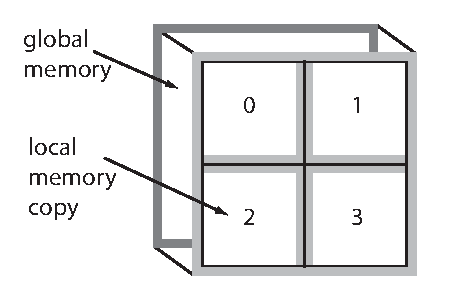
\includegraphics[width=1.75in]{cl-memory.pdf}
\caption{A schematic of global memory for an array and its copy stored in local memory
for four thread groups.}
\label{fig:cl-memory}
\end{figure}

We point out that the hierarchical distribution of memory used on the OpenCL
device shown in Figure~\ref{fig:cl-memory} is similar to the distribution of
memory across MPI nodes in an MPI application.  In the case of MPI, the
virtual global array is represented by the background layer (with its halo) and
partitions of the global array are stored in the 4 MPI nodes shown in the foreground.

Halo regions obtained via the {\tt region\_cpy} function (used with intent(in)
arrays) are constrained semantically so that they can not be written to by an
OpenCL kernel.  The {\tt region\_cpy} function returns a copy of the region of
the array stored in global memory and places it in local memory shared by
threads in a thread group.  Thus once memory for an array has been transferred
into global device memory by the host (before the OpenCL kernel is run), memory
is in a consistent state so that all kernel threads are free to read from global
device memory.  Because the local memory is a copy, it functions as a software
cache for the local thread group.  Thus the compiler must insert OpenCL barriers
at proper locations in the code to insure that all threads have written to the
local memory cache before any thread can start to read from the cache.  On exit
from a kernel, any local memory explicitly stored in register variables by the
compiler (memory accessed via the {\tt region\_cpy} function) is copied back to
global memory for all intent(out) arrays.  Recall that a thread may only write to
its own intent(out) array element, thus there are no race conditions when updating
intent(out) arrays.

%\subsection{ForOpenCL}

%This work describes transformations that automatically create OpenCL kernel
%functions from Fortran pure and elemental procedures.  At present, these transformations
%will not transform an entire program.  Users, for now, must explicitly replace
%calls to Fortran kernel procedures that run on the device, with calls to the
%OpenCL runtime that will run the kernel on the OpenCL host.  While these host
%transformations are straightforward using ROSE, they are outside the scope of
%this paper.

%In addition to the Fortran to OpenCL transformations, the
%ForOpenCL library available from the Open Fortran Parser web page provides programmers with the ability to
%call the C OpenCL runtime from Fortran.  ForOpenCL is a set of Fortran modules
%providing Fortran 2003 interface descriptions and classes that allow language
%interoperability with the OpenCL runtime.


\subsection{Transformation examples}

This section outlines the OpenCL equivalent syntax for portions of the Fortran
shallow-water code described in Section~\ref{sec:shallow-water}.  The notation
uses uppercase for arrays and lowercase for scalar quantities.  Variables
temporarily storing quantities for updated output arrays (declared as pointers
in Fortran) are denoted by a {\tt p} preceding the array name.  For example, the
Fortran statement {\tt pH = region\_ptr(oH, halo)} is transformed as a scalar
variable declaration representing a single element in the output array {\tt oH}.

\subsubsection{Region function}

While the Fortran version of the {\tt region\_cpy} function semantically returns
an array copy, in OpenCL this function returns a scalar quantity based on the
location of a thread in a thread group and the relationship of its location to
the array copy transferred to local memory.  Because we assume there is a thread
for every element in the interior, the array index is just the thread index
adjusted for the size of the halo.  Thus {\tt region\_cpy} is just an inline
OpenCL function and is provided by the ForOpenCL library.

\subsubsection{Function and variable declarations}

Fortran kernel procedures have direct correspondence with OpenCL equivalents.
For example, the {\tt wave\_advance} interface declaration is transformed as

{\small
\begin{verbatim}
__kernel void
wave_advance(float dx, ..., __global float * H, ...);
\end{verbatim}
}

The intent(in) arrays have local equivalents that are stored in local memory
and are declared by, for example,
{\small
\begin{verbatim}
__local float H_local[LOCAL_SIZE];
\end{verbatim}
}
\noindent
These local arrays are declared with the appropriate size and are
copied to local memory by the compiler with an inlined library function.  The
array temporaries defined on cell faces are declared similarly while interior
pointer variables are simple scalars, e.g., {\tt float pH}.  Intent(in) array
variables cannot be scalar objects because regions may be shifted and thus
\emph{shared} by threads within a thread group.

\subsubsection{Array syntax}

Array syntax transforms nearly directly to OpenCL code.  For example, interior
pointer variables are particularly straightforward as they are scalar quantities in
OpenCL,
{\small
\begin{verbatim}
pH = region_cpy(H, halo)
       + (dt/dx) * ( region_cpy(Ux, face_lt) -
                     region_cpy(Ux, face_rt) )
       + (dt/dy) * ( region_cpy(Vy, face_dn) -
                     region_cpy(Vy, face_up) );
\end{verbatim}
}
\noindent
Allocated variables are more complicated because they are arrays.
{\small
\begin{verbatim}
Hx[i] = 0.5 * (region(H_local, face_lt)+ ...);
\end{verbatim}
}
\noindent
where {\tt i = LX + LY*(NLX+halo(0)+halo(1)))} is a local index variable, {\tt
  LX = get\_local\_id(0)} is the local thread id in the $x$ dimension, {\tt LY =
  get\_local\_id(1)} is the local thread id in the $y$ dimension, {\tt NLX =
  get\_local\_size(0)} is the size of the thread group in the $x$ dimension, and
the {\tt get\_local\_id} and {\tt get\_local\_size} functions are defined by the
OpenCL language standard.

%\section{Static Analysis}
\label{sec:static-analysis}

1. Dependence analysis to insert thread group barriers

\begin{verbatim}
   barrier(CLK_LOCAL_MEM_FENCE)
\end{verbatim}

2. subsection variables associated with array variables

\subsection{Analysis not required}

1. loop fusion
2. removal of array temporaries (shifts)

\section{Performance Measurements}

It is important to note that the emphasis of this work is to explore and explain the new
syntax and execution semantics of a CAFe application.  A thorough examination of potential
performance gains (if any) using CAFe for parallelization of code is beyond the scope of
this paper.  The primary purpose of CAFe is to combine the parallel features of Fortran coarrays
--- executing a \emph{single} program --- with concurrent execution of separate tasks executing on
potentially heterogeneous hardware.

\begin{comment}
However, the relative performance of computation on a cluster of GPUs compared with the
necessary communication of halo information is of interest, especially considering that a
complete exchange of halo data involves communication between multiple coarray images
\emph{and} between each individual host image and its subimage (an attached OpenCL
device).
\end{comment}

However the relative performance of computation on the interior of a three-dimensional
grid, performed by the GPU, compared with the time required to compute on boundary planes by the
CPU is of interest.  Table 1 shows average execution time for a relaxation step on the GPU
(column 2) and on the CPU (column 3) in milliseconds, where $N$ (column 1) is the number of
cells in one dimension of a 3D cube; time for the exchange of halo information
between the GPU and the CPU for each iteration is also shown in column 4.

\begin{table}[]
\centering
\caption{Size of cube and time in milliseconds}
\label{table1}
\begin{tabular}{rrrrr}
$N$   &   GPU	 &  CPU         &   Comm    \\
      &   	 &              &           \\
16    &  0.02    &   0.01	&   0.07    \\
32    &  0.02    &   0.03       &   0.10    \\
64    &  0.04    &   0.12       &   0.27    \\
128   &  0.42    &   0.47	&   0.81    \\
256   &  4.59    &   1.97	&   2.99    \\
512   & 43.08    &   12.51	&  16.49    \\
\end{tabular}
\end{table}

Note that all three times in Table 1 are roughly equivalent for $N=128$.  Also note that
the communication and the computational times on the CPU are roughly equivalent and scale
the same with increasing $N$.  This is not surprising as both involve only the surface
elements of the cube.  However, computational time on the GPU grows much faster, O($N^3$),
as it is computing on the interior of the cube.

\begin{comment}
The current implementation does \emph{not} take advantage of optimization strategies such
as prefetching of array tiles (including halos) into OpenCL local memory.  Neither does it
take advantage of the potential of CAFe to overlap communication with computation (for
example, computing on ...
\end{comment}

\begin{comment}
Since many scientific codes are dominated by memory performance, including and especially
stencil algorithms as they typically only involve a computation on a small locally central
array element and a small overlapping halo region.  Stencil operations frequently do not
contain enough floating point operations per memory load to allow for floating point
performance to operate at peak (though this is entirely application and domain specific).
Thus we illustrate the \emph{potential} for performance by noting the latency and
throughput performance of an attached GPU in conjunction with MPI distributed memory
performance associated with halo transfer in Table 1.
\end{comment}

\begin{comment}
The results in Table 1 indicate that the primary bottleneck in using accelerators attached
to the TODO bus using OpenCL is likely to be the latency in transferring memory to and
from the device for distributed memory clusters of only a few nodes exchanging halo data
using MPI.
\end{comment}



\section{Conclusions}

The sheer complexity of programming for clusters of many or multi-core
processors with tens of millions threads of execution makes the simplicity of
the data-parallel model attractive.  The increasing complexity of
today's applications (especially in light of the increasing complexity
of the hardware) and the need for portability across architectures
make a higher-level and simpler programming model like data-parallel
attractive.

The goal of this work has been to exploit source-to-source transformations that
allow programmers to develop and maintain programs at a high-level of
abstraction, without coding to a specific hardware architecture.
Furthermore these transformations allow multiple hardware architectures
to be targeted without changing the high-level source.  It also removes the
necessity for application programmers to understand details of the accelerator
architecture or to know OpenCL.

%ACKNOWLEDGMENTS are optional
\section{Acknowledgments}
This work was supported in part by the Department of Energy Office of Science,
Advanced Scientific Computing Research.

%%TODO \cite{chamberlain04zpl, roth97stencils}

\bibliographystyle{abbrv}
\bibliography{local}

\balancecolumns
\end{document}
